\documentclass[11pt,a4paper]{article}
\usepackage{color}
\usepackage{graphicx}
\usepackage{sidecap}
\usepackage{mathtools}
%Om grotere integralen te krijgen
\usepackage{relsize}

%Andere breedte en lengthe van een document
\setlength{\textwidth}{6in} 
\addtolength{\hoffset}{-0.5in}
\setlength{\topmargin}{-0.2in}
\setlength{\textheight}{9in}

%Packages voor de figuren:
\usepackage{wrapfig}
\usepackage{caption}
\usepackage{subcaption}
%Kan er voor zorgen dat een figuur op de exacte plaats staat:
\usepackage{float}

\begin{document}
\begin{titlepage}
\title{\Huge Numerieke Wiskunde}
\author{Joni Allaert\\
		Ward Schodts\\
		}

\date{2013 - 2014}
\maketitle
\thispagestyle{empty}

\begin{center}


\includegraphics[scale=0.4]{KULzwart.png}

\end{center}
\begin{center}
\Large Professor Dr. ir. Marc Van Barel
\vfill
\end{center}
\end{titlepage}

\section{Deel 1: Numerieke integratie}
\subsection{Vast Deelinterval}
\subsubsection*{(a) Benadering van de integralen $\mathop{\mathlarger{\int\limits_{-1}^1e^xdx}}$ en  $\mathop{\mathlarger{\int\limits_{-5}^5\frac{1}{1+x^2}}}$}
\vspace{-20pt}
\begin{figure}[H]
	\begin{subfigure}{0.5\textwidth}
	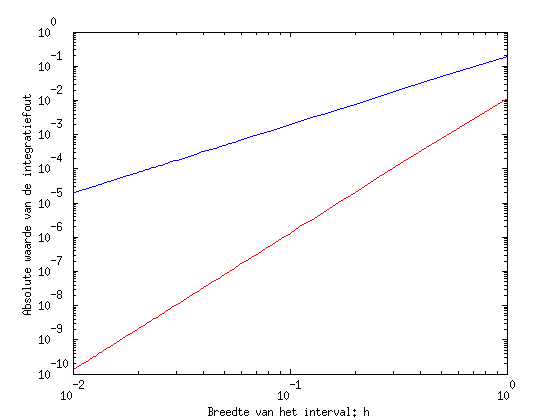
\includegraphics[width=\textwidth]{11a1.png}
	\caption*{$\int\limits_{-1}^1e^xdx$ met de trapeziumbenadering in het blauw en met de simpsonbenadering in het rood.}
	\end{subfigure}
	\hspace{10pt}
	%Laat hier geen lijnen tussen anders komen ze niet meer horizontaal gelijk
	\begin{subfigure}{0.5\textwidth}
	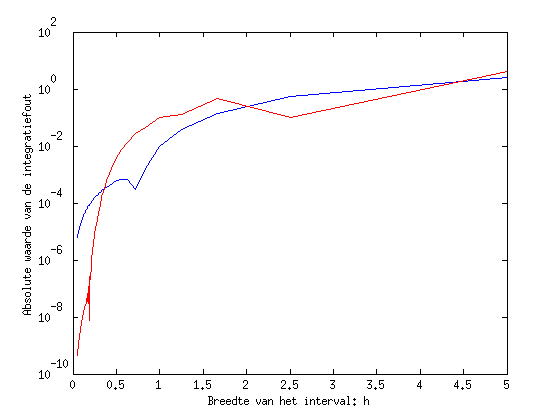
\includegraphics[width=\textwidth]{11a2.png}
	\caption*{$\int\limits_{-5}^5\frac{1}{1+x^2}$ met de trapeziumbenadering in het blauw en met de simpsonbenadering in het rood.}
	\end{subfigure}

\end{figure}

Om een duidelijk beeld te krijgen van de benaderingen, hebben we in het geval van de exponenti\"ele functie een loglog-plot genomen en voor de andere functie een semilogy-plot. Het doel was om de lijnen zo veel mogelijk te lineariseren. In het geval van de tweede functie was dit echter niet mogelijk.

\subsubsection*{(b) De waardes $k$ in $O(h^k$) voor de integratieregels}

De fout die veroorzaakt wordt bij de trapeziumregel gedraagt zich als $O(h^2)$. De verklaring hiervoor is dat de integratiefout bij de trapeziumregel te schrijven is als \[ F_n = -\dfrac{(b-a)^3}{12n^2}f^{(2)}(\eta) \] voor een $\eta \in (a,b)$. De fout gedraagt zich bijgevolg als $O(n^{-2})$. Wat hetzelfde is als $O(h^2)$, per definitie van $h$.
\\
De fout veroorzaakt door de regel van Simpson gedraagt zich als $O(h^4)$. We kunnen immers de integratiefout bij de Simpsonregel schrijven als \[ F_n = -\dfrac{(b-a)^5}{180n^4}f^{(4)}(\eta) \] voor een $\eta \in (a,b)$. De fout gedraagt zich dan als $O(n^{-4})$. Dit is, per definitie van $h$, hetzelfde als $O(h^4)$.
\vspace{-45pt}
\begin{figure}[H]
	\begin{subfigure}{0.5\textwidth}
	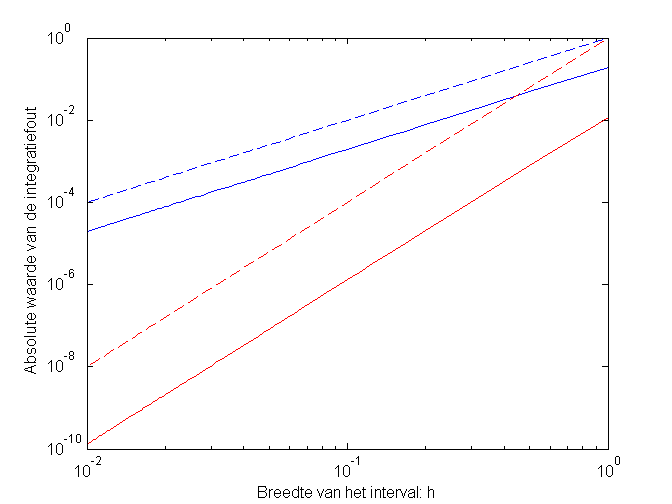
\includegraphics[width=\textwidth]{11b1.png}
	\caption*{$\int\limits_{-1}^1e^xdx$ het gedrag van de trapeziumbenadering met een blauwe stippellijn en het gedrag van de simpsonbenadering met een rode stippellijn.}
	\end{subfigure}
	\hspace{10pt}
	%Laat hier geen lijnen tussen anders komen ze niet meer horizontaal gelijk
	\begin{subfigure}{0.5\textwidth}
	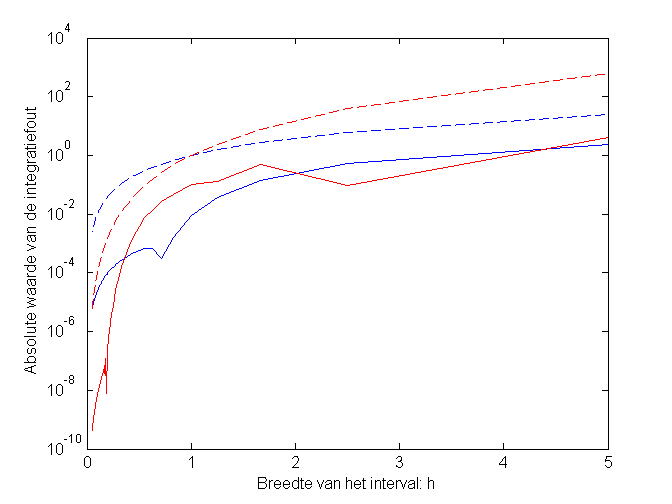
\includegraphics[width=\textwidth]{11b2.png}
	\caption*{$\int\limits_{-5}^5\frac{1}{1+x^2}$ het gedrag van de trapeziumbenadering met een blauwe stippellijn en het gedrag van de simpsonbenadering met een rode stippellijn.}
	\end{subfigure}

\end{figure}

\subsection{Adaptieve Routine}

\subsubsection*{(b) Het probleem bij $\mathop{\mathlarger{\int\limits_{-1}^1sin(2\pi x)^2dx}}$}

\begin{wrapfigure}{R}{0.4\textwidth}
	\begin{center}
	\vspace{-85pt}
	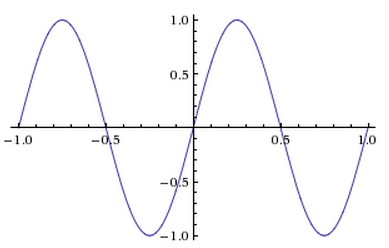
\includegraphics[width=0.5\textwidth]{12b.png}
	\caption*{$sin(2\pi x)^2dx$ van $-1$ tot $1$}
	\vspace{-25pt}
	\end{center}
	\end{wrapfigure}
We krijgen bij onze zelf gedefinieerde functies telkens waarden die nul benaderen i.p.v. de werkelijke waarde 1. Dit komt omdat we bij onze eerste recursiestap telkens gaan evalueren in een punt van de functie waar deze nul is. Zo evalueren we bij de trapeziummethode in de punten -1 en 1 voor $I_1$ en in de punten -1, 0 en 1 voor $I_2$. Net zoals we op de figuur kunnen zien is de functie telkens in deze waarden nul. Hierdoor is $I_1 - I_2$ ook een benadering van nul. Deze waarde is dan kleiner dan de tolerantie waardoor er maar 1 recursiestap wordt uitgevoerd en deze waarde wordt dan ook teruggegeven. Hetzelfde gebeurt bij de simpsonmethode waarvoor bij $I_1$ en $I_2$ respectievelijk in -1, 0, 1 en -1, -0.5, 0, 0.5, 1 wordt ge\"evalueerd. Om dit probleem op te lossen gaat \verb|quad| er voor zorgen dat er ongelijk deelintervallen zijn. Dat kan je zien in het volgende stuk code:
\begin{verbatim}
% Initialize with three unequal subintervals.
h = 0.13579*(b-a);
x = [a a+h a+2*h (a+b)/2 b-2*h b-h b];
\end{verbatim}
\subsubsection*{(c) Het probleem bij $\mathop{\mathlarger{\int\limits_{0}^1\frac{1}{\sqrt(x)}dx}}$}
Het probleem dat we hier krijgen is dat we de functie proberen te evalueren in punt waar hij niet gedefinieerd is. Namelijk het punt $x=0$. Hierdoor krijgen we een waarde $\infty$ voor zowel $I_1$ als $I_2$. Omdat er recursief altijd opnieuw wordt ge\"evalueerd wordt in $x=0$ dat telkens de waarde $\infty$ teruggeeft en bewerkingen hiermee ook $\infty$ teruggeven blijven we maar opnieuw recursief uitvoeren. Want de voorwaarde om met de recursie te stoppen: 
\verb|if abs(I1 - I2) < e| is nooit voldaan dan.
De methode \verb|quad| lost dit probleem op met volgende code:

\begin{verbatim}
% Fudge endpoints to avoid infinities.
if ~isfinite(y(1))
    y(1) = f(a+eps(superiorfloat(a,b))*(b-a),varargin{:});
    fcnt = fcnt+1;
end
if ~isfinite(y(7))
    y(7) = f(b-eps(superiorfloat(a,b))*(b-a),varargin{:});
    fcnt = fcnt+1;
end
\end{verbatim}
\verb|quad| checkt dus of de eindpunten niet oneindig zijn en als dit zo is dan word er een kleine waarde bij opgeteld of afgetrokken. Afhankelijk of het linkse of rechtse eindpunt van het interval, oneindig als waarde teruggeeft.
\subsubsection*{(d) De uitvoeringstijd in functie van e }

\begin{figure}[H]
	\vspace{-20pt}
	\centering
	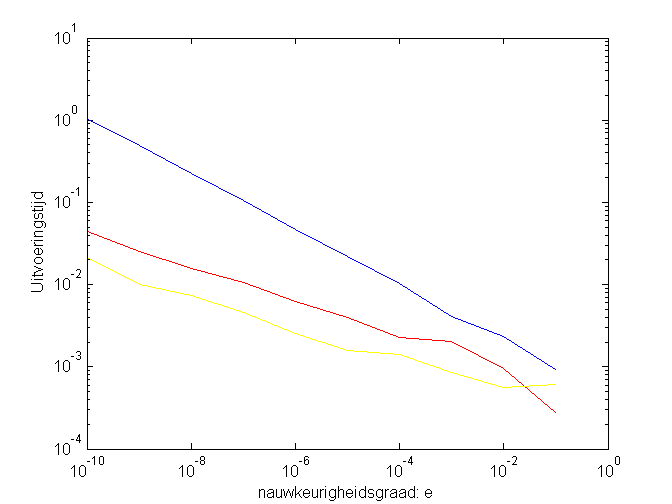
\includegraphics[width=0.7\textwidth]{12d1.png}
	\caption*{De uitvoeringstijden van trapezium, Simpson en quad in respectievelijke kleuren blauw, rood en geel.}
	\end{figure}
\subsubsection*{(e) Gedrag van de uitvoeringstijd in functie de naukeurigheid e}

We bepalen dit eerst voor de trapeziumregel. We veronderstellen de gegevens van in de opgave. De benaderde fout gedraagt zich in elk deelinterval dan als $O(h^3)$ (Dit kan men afleiden uit de theorie in het boek). Dus bij een verdubbeling van de graad $(n)$ deelt de fout door 8. Dit betekent dat we per iteratiestap net geen juist cijfer winnen $(log_{10}(8) = 0.9031)$. We verkrijgen dus in functie van $e$, $2^i$ deelintervallen met een constante uitvoeringstijd met $i =\dfrac{-log_{10}(e)}{log_{10}(8)}$ het aantal iteratiestappen. De uitvoeringstijd gedragt zich dan als $O(2^i)$
\\
\\
Voor Simpson en quad gedraagt de uitvoeringstijd zich op een constante na hetzelfde. We veronderstellen opnieuw de gegevens van in de opgave. De benaderde fout gedraagt zich in elk deelinterval dan als $O(h^5)$ (Dit kan men afleiden uit de theorie in het boek). Dus bij een verdubbeling van de graad $(n)$ deelt de fout door 32. Dit betekent dat we per iteratiestap net 1.5 juist cijfers winnen $(log_{10}(32) = 1.5051)$. We verkrijgen dus in functie van $e$ $2^i$ deelintervallen met een constante uitvoeringstijd met $i =\dfrac{-log_{10}(e)}{log_{10}(32)}$ het aantal iteratiestappen. De uitvoeringstijd gedragt zich dan als $O(2^i)$
\subsubsection*{(f) Grafieken samen met de theoretische uitvoeringstijd}
\begin{figure}[H]
	\vspace{-20pt}
	\centering
	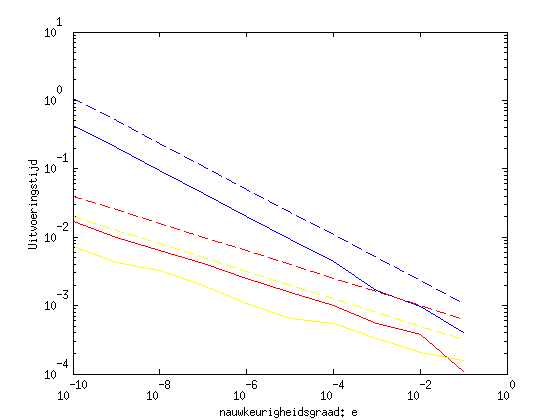
\includegraphics[width=0.7\textwidth]{12f.png}
	\end{figure}
De theoretische uitvoeringstijd bijgevoegd bij vorige figuur.
\section{Deel 2: Kleinste kwadraten benadering van een functie}

\subsection{Veeltermbenadering in monomiaalbasis}

\subsubsection*{(d) De fout $||f-g||$ in functie van de graad}
We hebben hier gekozen voor een semilogy-plot. Hier is immers het overgangspunt, waar de afbrekingsfouten het overnemen van de benaderingsfouten, het duidelijkst op te zien.
\begin{figure}[H]
\vspace{-35pt}
	\centering
	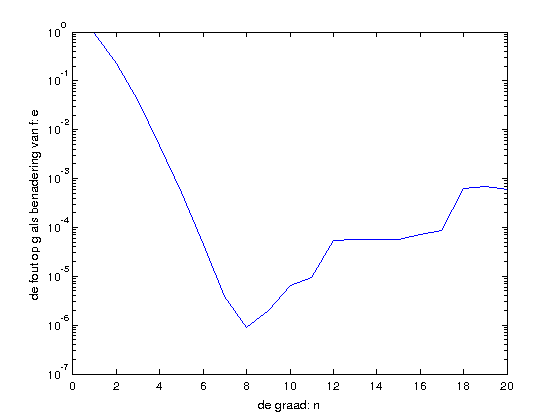
\includegraphics[width=0.7\textwidth]{22d1.png}
	\vspace{-10pt}
	\end{figure}

\subsubsection*{(e) Benaderings- of abrekingsfout?}

Het eerste, dalende deel is te wijten aan de benaderingsfouten. Dit stuk daalt, want als de graad stijgt kunnen we de functie steeds beter en beter benaderen. Vanaf een bepaald moment (hier bij een graad van 8) nemen echter de afbrekingsfouten de overhand en gaat de totale fout weer stijgen. Het stijgende tweede deel is dus te wijten aan afbrekingsfouten.
\vspace{-20pt}
\subsubsection*{(f) Convergentiesnelheid}

\begin{figure}[H]
	\centering
	\vspace{-20pt}
	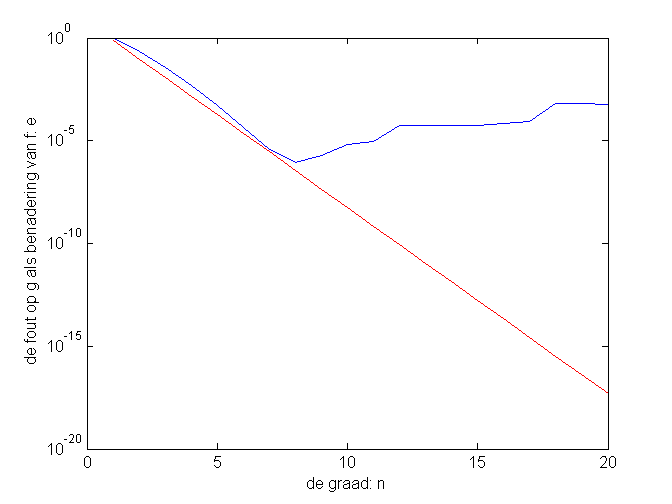
\includegraphics[width=0.7\textwidth]{22f1.png}
	\vspace{-15pt}
	\end{figure}
De convergentiesnelheid gedraagt zich als $O(8^{-n})$ met $n$ de graad van $g$.
\subsubsection*{(h) Perturbaties op A en b}
De groene lijn geeft aan waar $10^{-8}$ is. We kunnen dus duidelijk zien dat beide lijnen van grootteorde $10^{-8}$ zijn.
\begin{figure}[H]
	\centering
	\vspace{-30pt}
	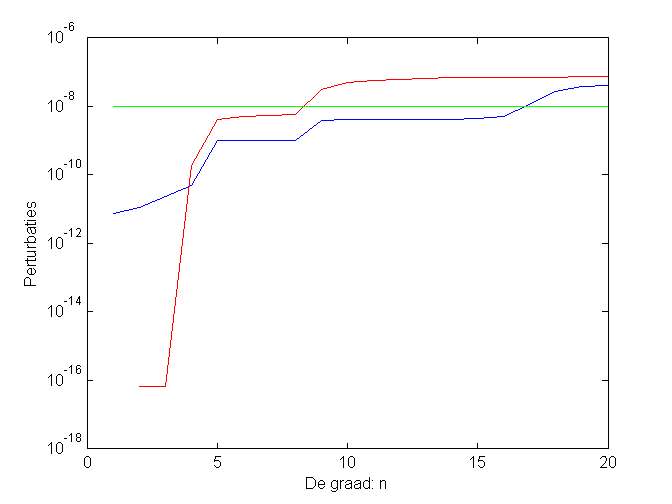
\includegraphics[width=0.7\textwidth]{22h1.png}
	\caption*{Perturbaties op A(rood), b(blauw)}
	\end{figure}
\vspace{-30pt}
\subsubsection*{(i) perturbatie op a}
\vspace{-20pt}
\begin{figure}[H]
	\centering
	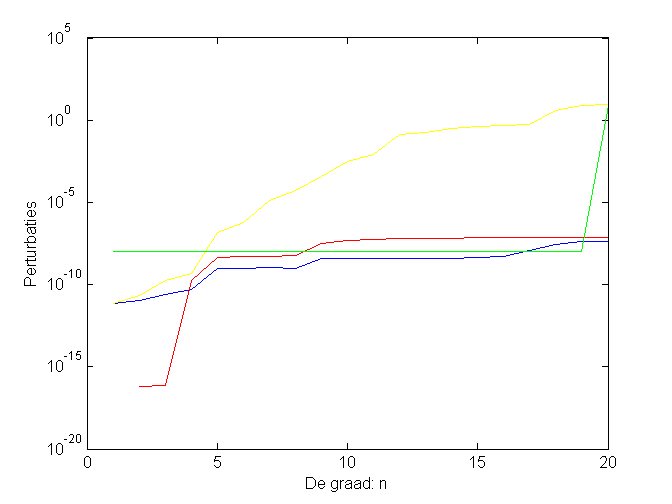
\includegraphics[width=0.7\textwidth]{22i1.png}
	\vspace{-10pt}
	\caption*{Perturbaties op a(geel) en tol vermenigvuldigd met het conditiegetal(groen) bijgevoegd bij de vorige grafiek.}
	\end{figure}
\vspace{-10pt}
De perturbaties op a stijgen logischerwijs systematisch naarmate dat de graad stijgt. De conditie van de matrix blijf lange tijd zeer goed, tot bij een graad tussen 18 en 19 waar de conditie ineens heel slecht wordt. Dit verklaart de plotse sprong van de groene lijn.
\vspace{-5pt}
\section{Tijdsbesteding}
\begin{center}
\begin{tabular}{ c || c }
Onderdeel & Tijdsbesteding\\
\hline
\hline
Doornemen opgave & 1u\\
\hline
Code deel 1 & 11u\\
\hline
Code deel 2 & 9u\\
\hline
Maken grafieken & 3u\\
\hline
Samenstellen verslag & 5u
\end{tabular}
\end{center}

\end{document}